\documentclass[fleqn]{article}
\usepackage{graphicx}
\usepackage{mathtools}
\mathtoolsset{showonlyrefs}
\usepackage{amsmath}
\usepackage{hyperref}
\DeclareGraphicsExtensions{.png}
\title{Verslag Project Codetheorie}
\date{2017-04-28}
\author{Sibert Aerts \and C\'{e}dric De Haes}

\begin{document}
	\maketitle
	
	\section{Vigen\`ere Plus}
	We zijn er in geslaagd de Vigen\`ere Plus code te kraken.\\
	We begonnen met het wiskundig uitschrijven van de gegeven encryptiemethode: Een Vigen\`ere versleuteling gevolgd door een enkele kolom transpositie. We merkten meteen dat er geen voor de hand liggende wiskundige of statistische oplossing was zolang de kolom sleutel (of tenminste de lengte hiervan) en de lengte van de Vigen\'ere sleutels onbekend waren.
	
	Om Vigen\`ere op te lossen analyseert men bepaalde attributen van de code: Het herhaaldelijke voorkomen van factoren in de afstanden tussen identieke substrings van 3 karakters, deze herhaalde factoren verklappen de lengte van de  Vigen\'ere sleutel. De kolom transpositie (of het omkeren van de transpositie met een foute sleutel) zorgt er echter voor dat deze onderliggende patronen verborgen blijven. Enkel als men een (quasi) juiste sleutel gebruikt om de kolom transpositie om te keren zal men een code verkrijgen waarin men zo patronen kan herkennen.
	
	Met dit in gedachte bedachten we een methode om een arbitraire sleutel $k$ een score te geven:
	\begin{enumerate}
		\setlength\itemsep{0pt}
		\item Gebruik de sleutel $k$ om de enkele kolomtranspositie ongedaan te maken.
		\item Analyseer de resulterende code en gebruik dit om een score te berekenen.
		\item Associ\"eer deze score met de sleutel $k$.
	\end{enumerate}
	Het berekenen van de score in stap 2 gebeurt aan de hand van een heuristiek, in dit geval bedachten we een simpele score functie: De som van elke factor maal het aantal voorkomens van die factor. We pasten deze methode toe op een grote hoeveelheid willekeurig gekozen sleutels met lengtes tussen 2 en 10. Uit de scores viel onmiddellijk op dat de sleutels met de hoogste scores lengte 7 hadden, wat aangeeft dat dit waarschijnlijk de correcte sleutellengte is.
	
	Nu kennen we echter enkel de lengte, en niet de sleutel zelf. Bij wijze van test namen we de hoogst scorende sleutel van lengte 7 (die zeker niet gegarandeerd was de juiste sleutel te zijn) en voegden het resultaat in de \textit{Vigen\`ere Cracking Tool} \footnote{\url{http://www.simonsingh.net/The_Black_Chamber/vigenere_cracking_tool.html}}. Deze gaf zeer duidelijk aan dat de Vigen\`ere sleutel lengte 14 moest zijn. Dit is een enorm behulpzaam feit want 14 is een veelvoud van 7, wat een speciale eigenschap geeft aan de combinatie Vigen\`ere en kolom transpositie:\\
	Neem:
	\begin{equation}
	\begin{aligned}
		& c = \text{ de correcte kolom sleutel (lengte 7)}\\
		& v = \text{de correcte Vigen\`ere sleutel (lengte 14)}	\\
		& text = \text{de originele text}\\
		& code = Col_{c} \circ Vig_{v} (text) = \text{de gegeven code}\\
		& c' = \text{een arbitraire kolom sleutel (lengte 7)} \\
		& v' = \text{de Vigen\`ere sleutel (lengte 14) gevonden aan de hand van } c' \\
		& text' = Vig_{v'}^{-1} \circ Col_{c'}^{-1} (code)
	\end{aligned}
	\end{equation}	
	Dan kan men aantonen dat omwille van de lengtes van $c$ en $v$:
	\begin{equation}
	\begin{aligned}
		&text' \text{ is een permutatie van } text\\
		&v' \text{ is een permutatie van } v\\
		&code' = Col_{c'}(text') = Col_{c'} \circ Vig_{v'}^{-1} \circ Col_{c'}^{-1} (code)\\
		& = Col_{c'} \circ Vig_{v'}^{-1} \circ Col_{c'}^{-1} \circ Col_{c} \circ Vig_{v} (text) \\
		& = Col_{c} (text)\\
	\end{aligned}
	\end{equation}	
	Kort gezegd: Het vinden van de meest waarschijnlijke Vigen\`ere sleutel voor een foute kolom sleutel die wel de juiste lengte heeft, staat ons toe om de Vigen`ere geheel teniet te doen. Het resultaat, $code'$, is een tekst die enkel versleuteld is met een kolom transpositie, en aangezien we de lengte van de sleutel kennen is het vinden van de oplossing hiervoor een simpele puzzel die we makkelijk manueel konden uitvoeren.\\\\	
	Uiteindelijk vonden we dus:
	\begin{itemize}
		\setlength\itemsep{0pt}
		\item De kolom sleutel: GBDAFCE
		\item De Vigen\`ere sleutel: SASKIADECOSTER
	\end{itemize}
	
	
	
	\section{PlayFair}
	Het is ons niet gelukt om de PlayFair code te kraken.\\
	We probeerden dit te doen met behulp van de frequentie-analyse van bigrammen. Eerst hebben we een playfair decoder ge\"{i}mplemeteerd. Deze gaat een code nemen en die decoderen volgens een gegeven vierkant. Deze hebben we nodig omdat de tekst te klein is om brute force de frequentie te nemen van elk bigram in de code te vervangen door het bigram met ongeveer gelijke frequentie. Daarom maken we in de start een random vierkant aan als sleutel en decoderen we de code met behulp van deze decoder. Dan wordt op deze gedecodeerde tekst een score geplakt. Deze score wordt berekend aan de hand van de frequentie-analyse gevonden op \\ \url{https://fusiontables.google.com/DataSource?docid=15jK-3WUD-JjQMdwLe-ipwqkUdjvf2JKK-D-s9as}\\
	Vanuit die tabel worden de frequenties van alle bigrammen berekend. De dubbele letters worden in deze tabel worden eerlijk verdeeld over beide mogelijkheden met een X. De frequenties van bigrammen met een J worden opgeteld met die van overeenkomstige bigrammen met een I.\\
	De score wordt berekend door de som te nemen van de frequenties in de gedecodeerde tekst.
	Deze score wordt dat vergeleken met de score van enkele andere dichtbijzijnde sleutels:
	\begin{enumerate}
		\item 1 rij omhoog
		\item 1 rij omlaag
		\item 1 rij links
		\item 1 rij rechts
		\item 1 rij spiegelen
		\item 1 kolom spiegelen
		\item 2 random rijen omwisselen
		\item 2 random kolommen omwisselen
		\item een random pair karakters omwisselen
		\item 5 random pair karakters omwisselen
		\item 2 random pair karakters omwisselen
		\item een random triplet omwisselen
	\end{enumerate}
	Als de score van van al deze sleutels kleiner is dan die van de oorspronkelijke sleutel, is de oorspronkelijke sleutel de correcte sleutel. Dit wordt dan nog een aantal keren herhaald omdat je werkt met random waardes. Als er een sleutel wordt gevonden met een betere of gelijke score, dan worden dichtbijzijnde sleutels bij die sleutel gekozen.\\
	Op deze manier kwamen we relatief snel aan een oplossing, maar was deze steeds incorrect. Toen bedachten we ons dat de letters die niet in het codewoord staan in alfabetische volgorde achter het codewoord geplaatst worden om het vierkant op te vullen. Dus voegden we de voorwaarde toe dat de laatste 5 karakters van de sleutel in alfabetische volgorde moeten staan. Dit komt niet uit voor codewoorden met meer dan 20 verschillende letters (J niet meegerekend). Daarom dat we aannemen dat de sleutel toch correct is als in dezelfde sleutel 100 keer naar een betere sleutel gezocht werd.
	\section{ADFVGX}
	Het is ons niet gelukt om de ADFVGX code te kraken.\\
	Onze aanpak was vergelijkbaar aan die voor de Vigen\`ere op te lossen: Eerst proberen de lengte van de kolom sleutel te vinden, en daarna proberen de eigenlijke ADFGVX substitutie te ontdekken. Net als bij de Vigen\`ere code begon deze aanpak met het opstellen van een score-functie voor het testen van de mogelijke correctheid van een sleutel die we willen gebruiken voor het omkeren van de kolom transpositie. Aangezien de interne encryptie niet langer Vigen\`ere is, maar een willekeurige mono-alfabetische substitutie, besloten we om niet dezelfde analyse te gebruiken. In de plaats daarvan hebben we gebruik gemaakt van data over de distributies van individuele letters in de gegeven talen (Engels, Duits, Frans en Nederlands), en gebruikten we de \textit{Mean Squared Error} om deze te vergelijken met de distributie die we vonden in de verkregen code.
	
	Door deze techniek wederom toe te passen op een grote hoeveelheid sleutels met lengtes tussen 2 en 10, merkten we dat de hoogst scorende sleutels allemaal lengte 7 hadden, en dat deze bovendien veel betere scores behaalden dan de beste sleutels van andere lengtes. We gingen er dus van uit dat de kolom sleutel lengte 7 had. E\'en sleutel stak er bovendien tussenuit, en zou mogelijk de correcte sleutel kunnen zijn: ``GFDBEAC''.
	
	We hadden echter geen uitsluitsel over de exacte sleutel voor de kolom transpositie, en met enkel de kennis over de lengte konden we deze keer niet zomaar de mono-alfabetische substitutie oplossen. Omdat bij ADFGVX elk teken naar 2 letters gesubstitueerd word zorgt dit er voor dat elk klein verschil in de veronderstelde kolom sleutel resulteert in een enorme verandering van het gedecodeerde bericht. Er was dus geen voor de hand liggende manier om vanuit dit punt de code geheel op te lossen.
	
	Een eerste mislukte strategie bestond er uit om te proberen de mono-alfabetische substitutie automatisch op te lossen door er van uit te gaan dat de gegeven tekst exact de distributie van zijn taal volgt. De bedoeling was om deze methode dan toe te passen op de reeks hoogst-scorende kolom sleutels, om dan manueel na te kijken of een van de resultaten op een tekst leek. Deze aanpak om een mono-alfabetische substitutie op te lossen is echter zeer na\"ief en gaf geen zinnige resultaten.
	
	Een andere strategie die we hadden bedacht, maar waar we niet de tijd voor hadden om deze tot werking te brengen, was om niet enkel na te gaan hoe goed de letterdistributies pasten aan die van de talen, maar om ook de distributies van \textit{combinaties} van letters te beschouwen. Met dit als doel hebben we tenminste nog geprobeerd om klinkers te identificeren, door het vinden van letters die naast vrijwel elke andere letter voorkomen, maar ook hier kwam weinig uit.\\\\	
	Ons incomplete, onzekere antwoord is tenslotte als volgt:
	\begin{itemize}
		\setlength\itemsep{0pt}
		\item De kolom sleutel: GFDBEAC
		\item Taal: Duits
	\end{itemize}
	
	\section{Enigma}
	Het is ons ook niet gelukt om de enigma code te kraken.\\
	Eerst hebben we een Enigma machine ge\"{i}mplementeerd. Met behulp van de code en de crib maakten we intern een graaf aan de hand van een dictionary van lijsten. Omdat we geen makkelijk algoritme ken om alle onafhankelijke cycles in een graaf te vinden. Omdat de graaf relatief klein is (24 paden) hebben we die manueel getekent en de cycles op deze figuur aangeduid. Zo bekwamen we volgende graaf. 
	\begin{figure}[h!]
		\centering
		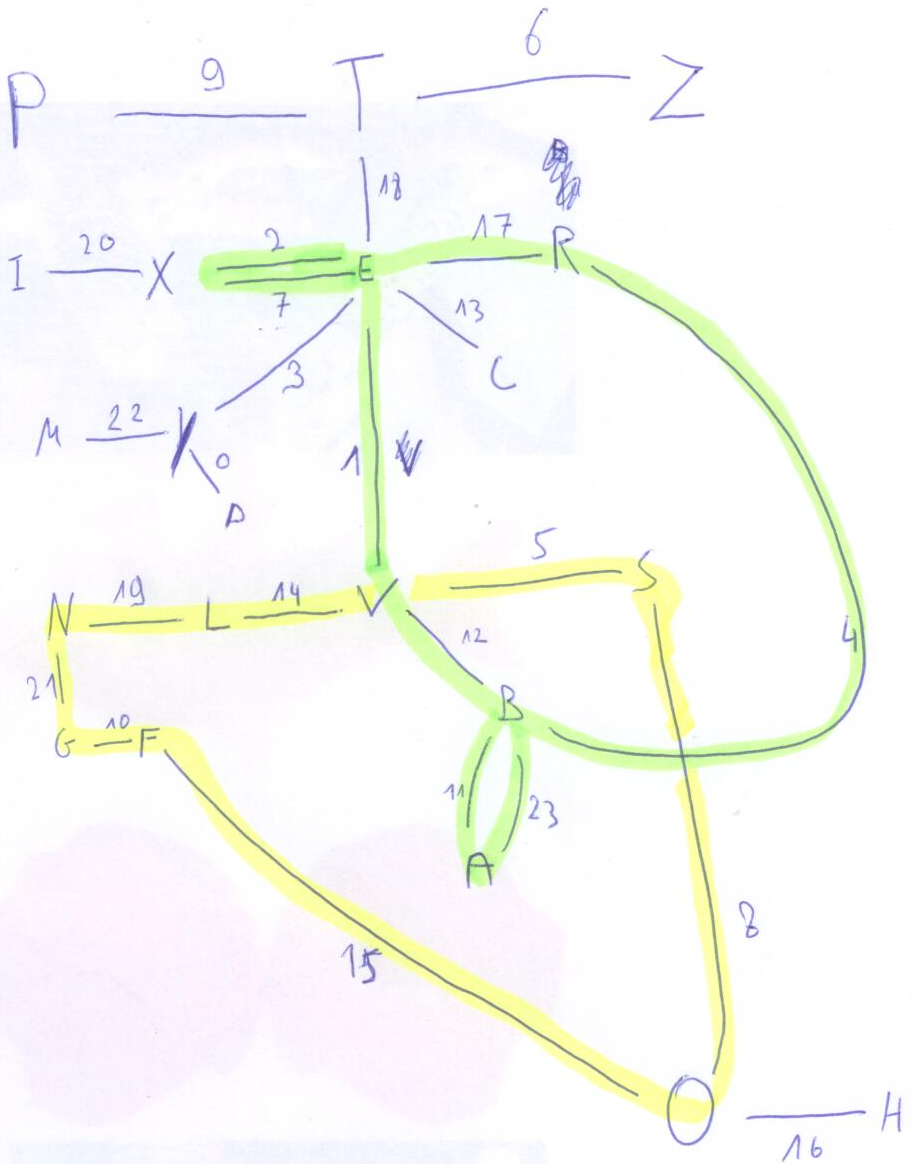
\includegraphics[width=0.5\linewidth]{Enigma}
		\caption[]{Enigma Graaf}
		\label{fig:enigma}
	\end{figure}

	Daaruit hebben we 4 onafhankelijke paden gevonden:
	\begin{enumerate}
		\item B $\rightarrow$ A $\rightarrow$ B
		\item E $\rightarrow$ X $\rightarrow$ E
		\item V $\rightarrow$ B $\rightarrow$ R $\rightarrow$ E $\rightarrow$ V
		\item V $\rightarrow$ S $\rightarrow$ O $\rightarrow$ F $\rightarrow$ G $\rightarrow$ N $\rightarrow$ L $\rightarrow$ V
	\end{enumerate}

	Er zijn dus fixpunten voor:
	\begin{enumerate}
		\item $\sigma \mathcal{E}_{k+11} \mathcal{E}_{k+23} \sigma$
		\item $\sigma \mathcal{E}_{k+2} \mathcal{E}_{k+7} \sigma$
		\item $\sigma \mathcal{E}_{k+5} \mathcal{E}_{k+8} \mathcal{E}_{k+15} \mathcal{E}_{k+10} \mathcal{E}_{k+21} \mathcal{E}_{k+19} \mathcal{E}_{k+14}\sigma$
		\item $\sigma \mathcal{E}_{k+12} \mathcal{E}_{k+4} \mathcal{E}_{k+17} \mathcal{E}_{k+1} \sigma$
	\end{enumerate}

	Deze hebben we dan manueel in onze kraker gestoken. Deze kraker probeert dan in alle mogelijke beginstanden een karakter te vinden die op zichzelf afbeelden door deze door de reeks van $\mathcal{E}_{k+i}$ te sturen. Omdat die nog altijd relatief veel mogelijkheden zullen zijn, gaan laten we daarna de ge\"{e}ncrypteerde tekst met die mogelijke beginstanden decoderen en kijken we of de tweede, derde en vierde letter dezelfde zijn. Die zullen gelijk zijn omdat deze letters gelijk zijn in de crib en het stekkerbord letters altijd op eenzelfde letter zal afbeelden. Dit dachten we dat het aantal mogelijkheden fel zou doen dalen en hebben we 's nachts op een server laten draaien.\\
	Daaruit bekwamen we nog altijd meer dan 300 mogelijkheden uit. Dit was te veel om met de hand na te kijken, dus lieten we er nog een check op uitvoeren.
	We laden de mogelijkheden in en gaan telkens een stekkerbord proberen te maken door te kijken naar de mapping van de crib tot de eerste letters van de gedecodeerde code. Daar mogen geen contradicties in zitten. Dit was jammer genoeg bij elke mogelijkheid wel het geval en uiteindelijk hadden we geen tijd meer om een andere oplossing te implementeren.
	\\
	Al de 327 mogelijkheden staan in de result.txt in de map Enigma. Het is telkens de setting van de Enigma machine gevolgd door de uitgeschreven code. Wat ons wel opviel was dat het vooral het 7de karakter (de vierde E) was die voor een fout zorgde in de mapping.
	
	
\end{document}